%%%%%%%%%%%%%%%%%%%%%%%%%%%%%%%%%%%%%%%%%
% Homework Assignment Article
% LaTeX Template
% Version 1.3.1 (ECL) (08/08/17)
%
% This template has been downloaded from:
% Overleaf
%
% Original author:
% Victor Zimmermann (zimmermann@cl.uni-heidelberg.de)
%
% License:
% CC BY-SA 4.0 (https://creativecommons.org/licenses/by-sa/4.0/)
%
%%%%%%%%%%%%%%%%%%%%%%%%%%%%%%%%%%%%%%%%%

%----------------------------------------------------------------------------------------

\documentclass[a4paper]{article} % Uses article class in A4 format

%----------------------------------------------------------------------------------------
%	FORMATTING
%----------------------------------------------------------------------------------------

\addtolength{\hoffset}{-2.25cm}
\addtolength{\textwidth}{4.5cm}
\addtolength{\voffset}{-3.25cm}
\addtolength{\textheight}{5cm}
\setlength{\parskip}{0pt}
\setlength{\parindent}{0in}

%----------------------------------------------------------------------------------------
%	PACKAGES AND OTHER DOCUMENT CONFIGURATIONS
%----------------------------------------------------------------------------------------

\usepackage{blindtext} % Package to generate dummy text
% \usepackage[style=numeric,sorting=none]{biblatex}
\usepackage{charter} % Use the Charter font
\usepackage[utf8]{inputenc} % Use UTF-8 encoding
\usepackage{microtype} % Slightly tweak font spacing for aesthetics

\usepackage[english]{babel} % Language hyphenation and typographical rules

\usepackage{amsthm, amsmath, amssymb} % Mathematical typesetting
\usepackage{float} % Improved interface for floating objects
\usepackage[final, colorlinks = true, 
            linkcolor = black, 
            citecolor = black]{hyperref} % For hyperlinks in the PDF
\usepackage{graphicx, multicol} % Enhanced support for graphics
\usepackage{xcolor} % Driver-independent color extensions
\usepackage{marvosym, wasysym} % More symbols
\usepackage{rotating} % Rotation tools
\usepackage{censor} % Facilities for controlling restricted text
\usepackage{listings, style/lstlisting} % Environment for non-formatted code, !uses style file!
\usepackage{pseudocode} % Environment for specifying algorithms in a natural way
\usepackage{style/avm} % Environment for f-structures, !uses style file!
\usepackage{booktabs} % Enhances quality of tables

\usepackage{tikz-qtree} % Easy tree drawing tool
\tikzset{every tree node/.style={align=center,anchor=north},
         level distance=2cm} % Configuration for q-trees
\usepackage{style/btree} % Configuration for b-trees and b+-trees, !uses style file!

% \usepackage[backend=biber,style=numeric,
            % sorting=nyt]{biblatex} % Complete reimplementation of bibliographic facilities
% \addbibresource{ecl.bib}
\usepackage{csquotes} % Context sensitive quotation facilities

\usepackage[yyyymmdd]{datetime} % Uses YEAR-MONTH-DAY format for dates
\renewcommand{\dateseparator}{-} % Sets dateseparator to '-'

\usepackage{fancyhdr} % Headers and footers
\pagestyle{fancy} % All pages have headers and footers
\fancyhead{}\renewcommand{\headrulewidth}{0pt} % Blank out the default header
\fancyfoot[L]{School of Computing, Macquarie University} % Custom footer text
\fancyfoot[C]{} % Custom footer text
\fancyfoot[R]{\thepage} % Custom footer text

\usepackage{comment}
\newcommand{\note}[1]{\marginpar{\scriptsize \textcolor{red}{#1}}} % Enables comments in red on margin

%----------------------------------------------------------------------------------------

\begin{document}

%----------------------------------------------------------------------------------------
%	TITLE SECTION
%----------------------------------------------------------------------------------------

\title{COMP3100 project report} % Article title
\fancyhead[C]{}
\hrule \medskip % Upper rule
\begin{minipage}{1\textwidth} % Center of title section
\centering 
\large % Title text size
Project report: Stage 2\\ % Assignment title and number
COMP3100 Distributed Systems, S1, 2023\\
\normalsize % Subtitle text size
SID: 46293175, Name: Quoc Huy Pham
%%%%\\ % Assignment subtitle
\end{minipage}
\medskip\hrule % Lower rule
\bigskip

%----------------------------------------------------------------------------------------
%	ARTICLE CONTENTS
%----------------------------------------------------------------------------------------
\section{Introduction}

This report focuses on designing a new job dispatching algorithm using the client created in the previous stage of the project. The new algorithm must be able to schedule jobs that optimise
average turnaround time without sacrificing too much resource utilisation and server rental cost.
\\This project is a minor part of a more significant project for unit COMP3100, in which students have to develop a custom job dispatcher algorithm that satisfies the previously mentioned conditions.
\\The stage 2 project, which is what this report is written for, will focus on creating a new algorithm and optimising it to achieve the previously mentioned, alongside improving the client itself in terms of code elegance, redundancy and readability.

\section{Problem Definition}
\label{sec:section2}

This section will cover the problem definition of this stage of the project. As stated by the specification of this stage: the objectives are incompatible (conflicting performance objectives), meaning optimising one aspect (turnaround time) may imply sacrificing the optimisation of other measures (resources). Because of that, the new algorithm must strike a balance between the objectives.\\
In summary, the problem this stage requires us to solve is determining how we can make an algorithm that can satisfy all objectives without tilting over a certain side. In the case of multiple algorithms, determine how each algorithm focuses on what aspect of the objective and the reason for it to be the case.

\section{The First-Fit/Best-Fit Hybrid Algorithm (FFBFH)}
\label{sec:section3}
\subsection{Algorithm Explanation}
First-Fit/Best-Fit Hybrid algorithm (FFBFH), as the name suggests, is a custom algorithm that tries to merge the best of the First-Fit algorithm (FF) and Best-Fit algorithm (BF) implemented by \href{https://github.com/distsys-MQ/ds-sim}{ds-client and ds-server} \cite{ds-sim} that follows the schedule rules of FF with some extra flags based on BF.\\
FFBFH follows the principle of FF: searches servers from the beginning to the end of the server list and assigns jobs to the server that first fits the job's criteria. Otherwise, regardless of availability, it assigns the job to the first fit server with sufficient initial resource capacity. FFBFH adds additional "fitness" criteria to help improve resource utilisation and turnaround time, \href{https://www.tutorialspoint.com/operating_system/os_memory_allocation_qa2.htm}{a huge disadvantage} \cite{mem-allocation} that has been known with FF, without trading too much turnaround time. The "fitness" criteria are determined through the usage of the "fitness" coefficient. This coefficient is calculated with a simple math equation:

\begin{figure}[h!]
    \centering
    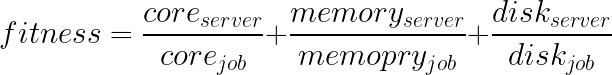
\includegraphics[scale = 0.5]{img/fitness.png}
    \caption{fitness equation}
    \label{fig:fig1}
\end{figure}
where:
\begin{itemize}
    \item server: the server that is available for scheduling
    \item job: the job that needs to be scheduled
\end{itemize}
This equation is based on BF's server selection rule that uses the server's core count to determine whether a server is fitted to do the job. "fitness" equation expands that rule so it combines the disk usage and memory into the rule, which in theory should provide better resource usage while improving turnaround time. The lower the "fitness" value, the more suitable that server is to do the job.\\
The algorithm will ask \href{https://github.com/distsys-MQ/ds-sim}{ds-server} \cite{ds-sim} to get servers that are capable of doing the job immediately. If there are servers that can do it immediately, the first one sent to the client will be selected to schedule the job. If there aren't any servers that can execute the job immediately, the algorithm will instead use servers that will "eventually" be capable of executing the job. At this stage, the equation shown in Figure \ref{fig:fig1} will be used to filter what server will be selected to execute the job. If two or more servers have the same fitness value, the server's cores will then be used as a backup filter. Again, if there are suitable servers with the same core count, their ID will then be used as the final effort to select the best server.\\
the following diagram will help visualise the process of scheduling using the FFBFH algorithm:
\begin{figure}[h!]
    \centering
    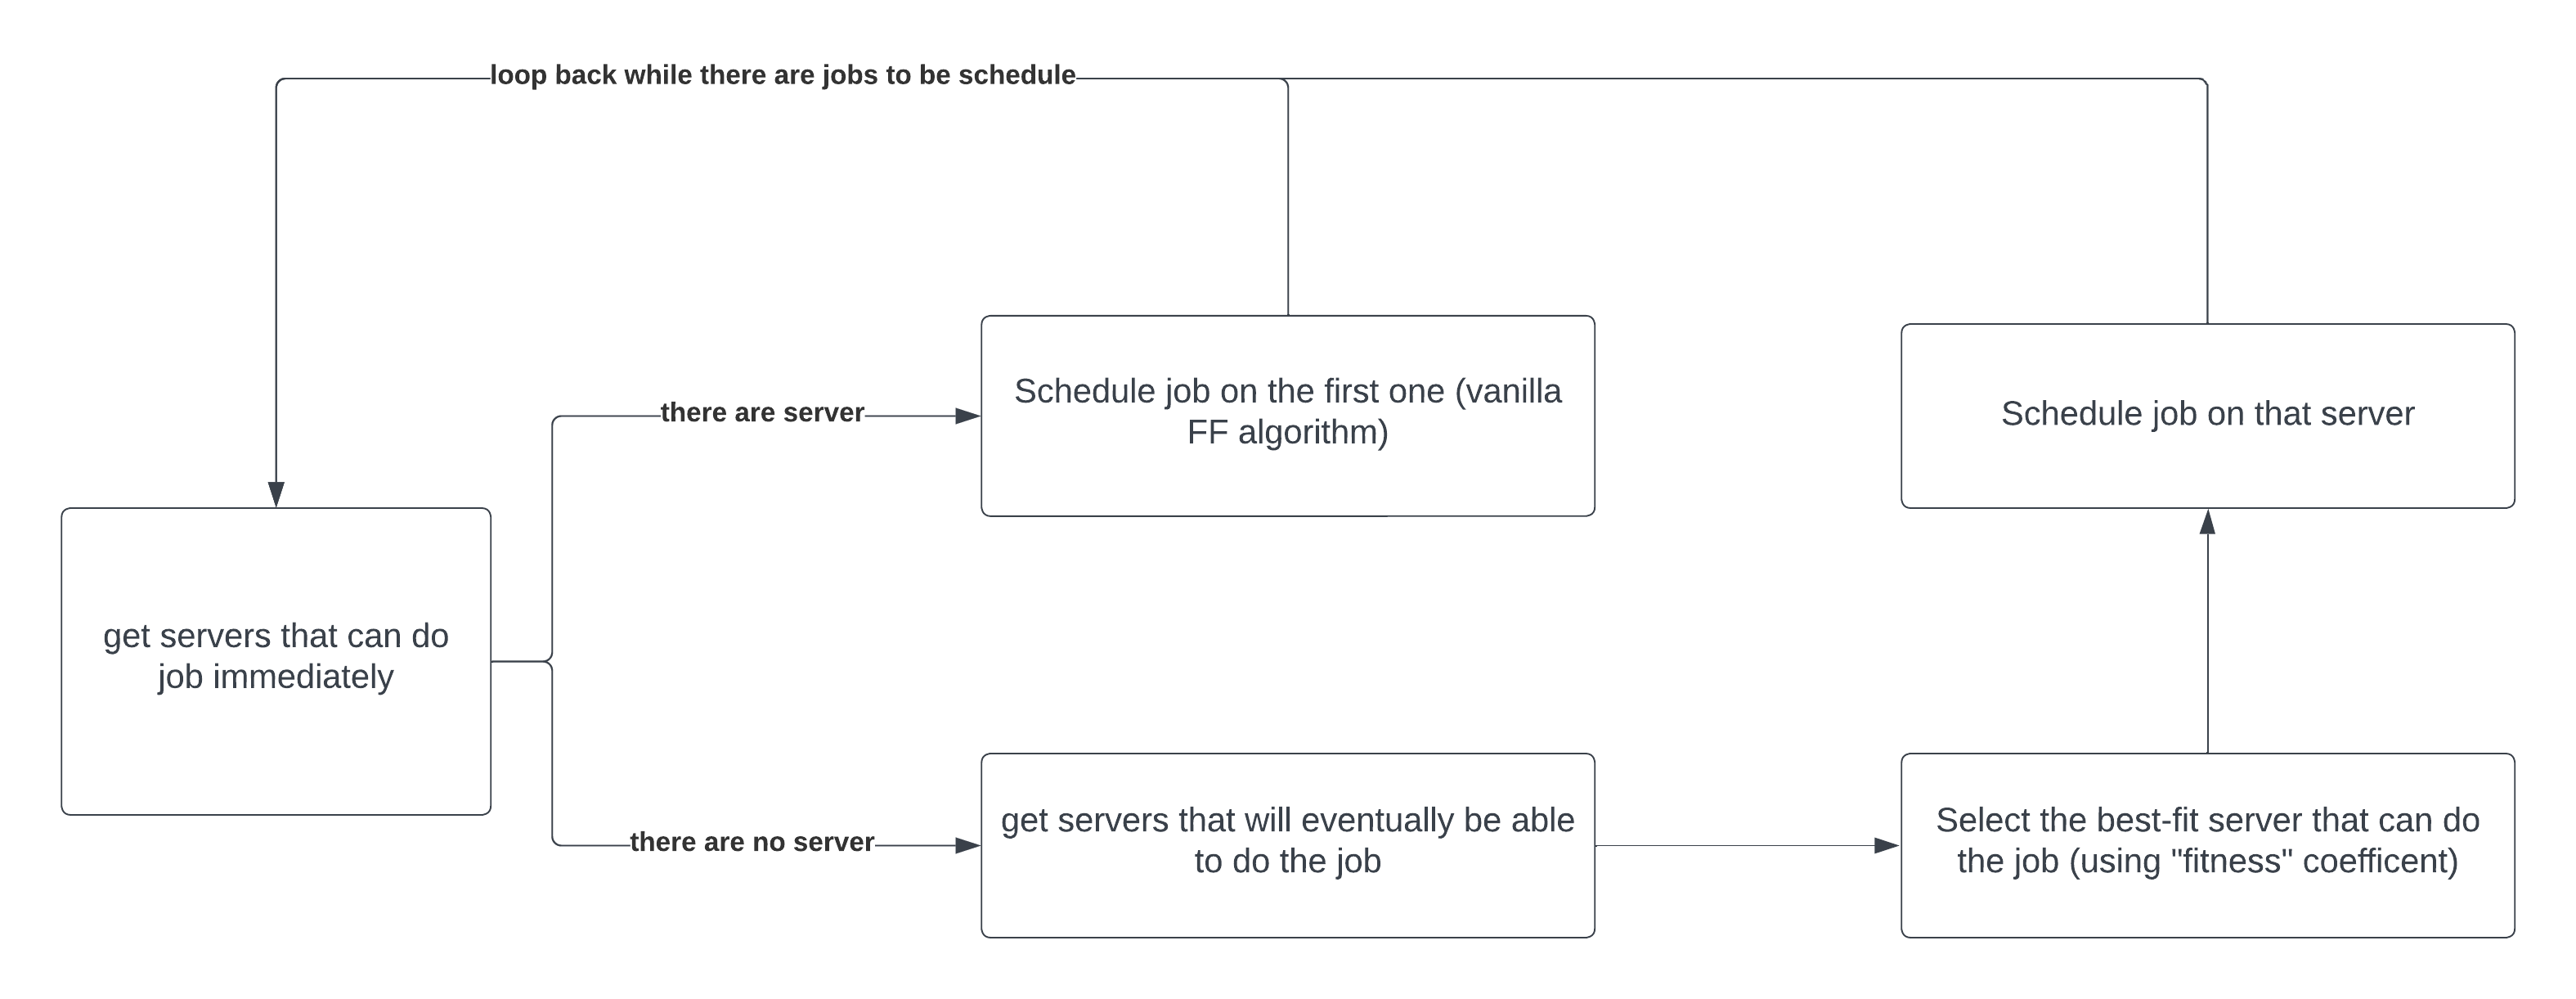
\includegraphics[scale = 0.125]{img/algorithm.png}
    \caption{FFBFH algorithm}
    \label{fig:fig2}
\end{figure}
\subsection{Sample screnario}
The following is a simple config to illustrate how the algorithm will work:
\begin{lstlisting}[breaklines]
<?xml version="1.0" encoding="UTF-8"?>
<!-- generated by: Y. C. Lee -->
<config randomSeed="1024">   
  <servers>
	<server type="juju" limit="2" bootupTime="60" hourlyRate="0.2" cores="2" memory="4000" disk="16000" />
	<server type="joon" limit="2" bootupTime="60" hourlyRate="0.4" cores="4" memory="16000" disk="64000" />
	<server type="super-silk" limit="1" bootupTime="80" hourlyRate="0.8" cores="16" memory="64000" disk="512000" />
  </servers>
  <jobs>
	<job type="short" minRunTime="1" maxRunTime="300" populationRate="60" />
	<job type="medium" minRunTime="301" maxRunTime="1800" populationRate="30" />
	<job type="long" minRunTime="1801" maxRunTime="100000" populationRate="10" />
  </jobs>
  <workload type="moderate" minLoad="30" maxLoad="70" />
  <termination>
	<condition type="endtime" value="604800" />
	<condition type="jobcount" value="10" />
  </termination>
</config> 
\end{lstlisting}

Initially, the client sends to ds-server to get available servers that can do jobs immediately. ds-server replies with a list of servers that can do that. The client then picks the first one:
\begin{lstlisting}
server recieve : GETS Avail 3 700 3800

server send : DATA 3 124
server recieve : OK

server send : joon 0 inactive -1 4 16000 64000 0 0
server send : joon 1 inactive -1 4 16000 64000 0 0
server send : super - silk 0 inactive -1 16 64000 512000 0 0
server recieve : OK

server send : .
server recieve : SCHD 0 joon 0

server send : OK
server recieve : REDY
\end{lstlisting}

If there are no servers that can do the job immediately, the client then sends to ds-server a request to get a list of servers that will eventually be able to do the job. After getting the servers, the "fitness" coefficient will be used to select the one best-fitted for the job (in this case, it's joon 0).

\begin{lstlisting}
server recieve: GETS Avail 4 4000 7600

server send: DATA 0 124
server recieve: OK

server recieve: GETS Capable 4 4000 7600

server send: .
server send: DATA 3 124
server recieve: OK

server send: joon 0 active 97 0 15200 58200 0 2
server send: joon 1 active 161 2 15100 61500 0 1
server send: super-silk 0 booting 236 13 61300 509400 1 0
server recieve: OK

server send: .
server recieve: SCHD 6 joon 0

server send: OK
server recieve: REDY
\end{lstlisting}
\section{Algorithm evaluation}
\label{sec:section4}
The average results collected from week 11's sample configuration is used for this evaluation.
\subsection{Turnaround time}
\begin{lstlisting}
Config                      |FF        |BF        |FFQ       |BFQ       |WFQ       |FFBFH
Average                     |1867.13   |2417.27   |2559.07   |2401.80   |9958.40   |1405.60   
Normalised (FF)             |1.0000    |1.2946    |1.3706    |1.2864    |5.3335    |0.7528    
Normalised (BF)             |0.7724    |1.0000    |1.0587    |0.9936    |4.1197    |0.5815    
Normalised (FFQ)            |0.7296    |0.9446    |1.0000    |0.9385    |3.8914    |0.5493    
Normalised (BFQ)            |0.7774    |1.0064    |1.0655    |1.0000    |4.1462    |0.5852    
Normalised (WFQ)            |0.1875    |0.2427    |0.2570    |0.2412    |1.0000    |0.1411    
Normalised (Average)        |0.4861    |0.6294    |0.6663    |0.6253    |2.5928    |0.3660
\end{lstlisting}
The average turnaround time is 1405.6 seconds, which is the fastest out of all baseline algorithm. Comparing normalised data, FFBFH is around:
\begin{itemize}
    \item 24.72 percent faster than FF
    \item 41.85 percent faster than BF
    \item 45.07 percent faster than FFQ
    \item 41.48 percent faster than BFQ
    \item 85.89 percent faster than WFQ
    \item On average, FFBFH is 63.4 percent faster
\end{itemize}
\subsection{Resource utilisation}
\begin{lstlisting}
Config                      |FF        |BF        |FFQ       |BFQ       |WFQ       |FFBFH
Average                     |74.02     |69.55     |73.49     |69.45     |68.18     |74.54     
Normalised (FF)             |1.0000    |0.9396    |0.9928    |0.9382    |0.9211    |1.0070    
Normalised (BF)             |1.0642    |1.0000    |1.0566    |0.9985    |0.9802    |1.0717    
Normalised (FFQ)            |1.0072    |0.9465    |1.0000    |0.9450    |0.9278    |1.0143    
Normalised (BFQ)            |1.0659    |1.0015    |1.0582    |1.0000    |0.9817    |1.0733    
Normalised (WFQ)            |1.0857    |1.0202    |1.0779    |1.0186    |1.0000    |1.0933    
Normalised (Average)        |1.0435    |0.9805    |1.0360    |0.9790    |0.9611    |1.0508   
\end{lstlisting}
The average resource utilisation is 74.54 percent, which is the best out of all baseline algorithm. Comparing normalised data, FFBFH is around:
\begin{itemize}
    \item 0.70 percent faster than FF
    \item 7.17 percent faster than BF
    \item 1.43 percent faster than FFQ
    \item 7.33 percent faster than BFQ
    \item 9.33 percent faster than WFQ
    \item On average, FFBFH is 5.08 percent faster
\end{itemize}
\subsection{Rental cost}
\begin{lstlisting}
Config                      |FF        |BF        |FFQ       |BFQ       |WFQ       |FFBFH
Average                     |526.40    |524.82    |537.31    |531.21    |555.13    |526.72    
Normalised (FF)             |1.0000    |0.9970    |1.0207    |1.0091    |1.0546    |1.0006    
Normalised (BF)             |1.0030    |1.0000    |1.0238    |1.0122    |1.0578    |1.0036    
Normalised (FFQ)            |0.9797    |0.9767    |1.0000    |0.9886    |1.0332    |0.9803    
Normalised (BFQ)            |0.9909    |0.9880    |1.0115    |1.0000    |1.0450    |0.9915    
Normalised (WFQ)            |0.9483    |0.9454    |0.9679    |0.9569    |1.0000    |0.9488    
Normalised (Average)        |0.9840    |0.9810    |1.0044    |0.9930    |1.0377    |0.9846    
\end{lstlisting}
The average rental cost is 526.72 dollars, which is the third best out of all baseline algorithm; beating by BF at 524.82 dollars and FF at 526.40 dollars. Comparing normalised data, FFBFH is around:
\begin{itemize}
    \item 0.07 percent slower than FF
    \item 0.36 percent slower than BF
    \item 1.97 percent faster than FFQ
    \item 0.85 percent faster than BFQ
    \item 5.12 percent faster than WFQ
    \item On average, FFBFH is 1.54 percent faster
\end{itemize}
\section{Sumary}
\label{sec:section5}
In summary, FFBFH has successfully achieved its goal of negating FF's disadvantage without creating a significant negative impact on other aspects. Although some trade-offs need to be made, especially with rental cost in certain configs, the benefits it brings in terms of turnaround time (over 63 percent faster than the 3 baseline algorithms) outweigh the negative effect on rental cost.\\
Further optimisations can also be applied to make the algorithm works even better in every aspect. A few of those optimisations include shutting down idle servers, implementing a global queuing system and newer and stricter rulesets.
\section{Github link}
https://github.com/Fozzyishere/COMP3100.git
%----------------------------------------------------------------------------------------
%	REFERENCE LIST
%----------------------------------------------------------------------------------------
\bibliographystyle{ieeetr}
\bibliography{comp3100project}
% \printbibliography
\bibitem[]{}
%----------------------------------------------------------------------------------------

\end{document}
